% !TeX root = origami-math.tex

\chapter{Axioms}\label{c.axioms}

\section{Axiom 1}\label{s.ax1}


\textbf{Axiom} 
Given two distinct points $p_1=(x_1,y_1)$, $p_2=(x_2,y_2)$, there is a unique fold $l$ that passes through both of them.

%\begin{figure}[H]
\begin{center}
\begin{tikzpicture}[scale=1.2]
\draw[step=10mm,white!50!black,thin] (-1,-1) grid (8,6);
\draw[thick] (-1,0) -- (8,0);
\draw[thick] (0,-1) -- (0,6);
\foreach \x in {0,...,8}
  \node at (\x-.2,-.2) {\sm{\x}};
\foreach \y in {1,...,6}
  \node at (-.2,\y-.3) {\sm{\y}};
\coordinate (P1) at (2,2);
\coordinate (P2) at (6,4);
\draw[very thick,dashed] ($(P1)!-.75!(P2)$) -- node[very near end,below] {$l$} ($(P1)!1.5!(P2)$);
\fill (P1) circle(2pt) node[above left] {$p_1$};
\fill (P2) circle(2pt) node[above left] {$p_2$};

\draw[very thick,dotted,->,bend left=30] (2,5) to (4,1);
\end{tikzpicture}
\end{center}
%\end{figure}

\textbf{Derivation of the equation of the fold}

The equation of fold $l$ is derived from the coordinates of $p_1$ and $p_2$: the slope is the quotient of the differences of the coordinates and the intercept is derived from $p_1$:
\begin{equation}
y - y_1 = \disfrac{y_2-y_1}{x_2-x_1}(x-x_1)\,.
\end{equation}

\vspace*{-3ex}
%\newpage

\textbf{Example}

Let  $p_1=(2,2), p_2=(6,4)$. The equation of $l$ is:
\begin{form}{2}
y-2&=&\disfrac{4-2}{6-2}(x-2)\\
y&=&\disfrac{1}{2}x+1\,.
\end{form}

%%%%%%%%%%%%%%%%%%%%%%%%%%%%%%%%%%%%%%%%%%%%%%%%%%%%%%%%%%%%%%%%
\newpage

\section{Axiom 2}\label{s.ax2}


\textbf{Axiom} 
Given two distinct points $p_1=(x_1,y_1)$, $p_2=(x_2,y_2)$, there is a unique fold $l$ that places $p_1$ onto $p_2$.

%\begin{figure}[H]
\begin{center}
\begin{tikzpicture}[scale=1.2]
\draw[step=10mm,white!50!black,thin] (-1,-1) grid (8,6);
\draw[thick] (-1,0) -- (8,0);
\draw[thick] (0,-1) -- (0,6);
\foreach \x in {0,...,8}
  \node at (\x-.2,-.2) {\sm{\x}};
\foreach \y in {1,...,6}
  \node at (-.2,\y-.3) {\sm{\y}};
\coordinate (P1) at (2,2);
\coordinate (P2) at (6,4);
\coordinate (mid1) at ($(P1)!.5!(P2)$);
\coordinate (mid2) at ($(P1)!.5!(P2)+(-1,2)$);

\draw[rotate=30] (mid1) rectangle +(8pt,8pt);

\draw[very thick,dotted] (P1) -- (P2);
\draw[very thick,dashed] ($(mid1)!-1.4!(mid2)$) -- node[very near end,left,yshift=-12pt] {$l$} ($(mid1)!1.4!(mid2)$);
\fill (P1) circle(2pt) node[above left] {$p_1$};
\fill (P2) circle(2pt) node[above left] {$p_2$};

\draw[very thick,dotted,->,bend right=50] (2,1.8) to (6,3.8);
\end{tikzpicture}
\end{center}
%\end{figure}

\textbf{Derivation of the equation of the fold}

The line $l$ is the perpendicular bisector of $\overline{p_1p_2}$. Its slope is the negative inverse of the slope of the line connecting $p_1$ and $p_2$. The line passes through the midpoint between the points:
\begin{equation}
y - \disfrac{y_1+y_2}{2} = -\disfrac{x_2-x_1}{y_2-y_1}\left(x-\disfrac{x_1+x_2}{2}\right)\,.\label{eq.midpoint1}
\end{equation}

\textbf{Example}

Let $p_1=(2,2), p_2=(6,4)$. The equation of $l$ is:
\begin{form}{2}
y-\left(\disfrac{2+4}{2}\right)&=&-\disfrac{6-2}{4-2}\left(x-\left(\disfrac{2+6}{2}\right)\right)\\
y&=&-2x+11\,.
\end{form}

%%%%%%%%%%%%%%%%%%%%%%%%%%%%%%%%%%%%%%%%%%%%%%%%%%%%%%%%%%%%%%%%
\newpage

\section{Axiom 3}\label{s.ax3}


\textbf{Axiom} 
Given two lines $l_1$ and $l_2$, there is a fold $l$ that places $l_1$ onto $l_2$.

%\begin{figure}[H]
\begin{center}
\begin{tikzpicture}[scale=1.2]
\draw[step=10mm,white!50!black,thin] (-1,-1) grid (8,7);
\draw[thick] (-1,0) -- (8,0);
\draw[thick] (0,-1) -- (0,7);
\foreach \x in {0,...,8}
  \node at (\x-.2,-.2) {\sm{\x}};
\foreach \y in {1,...,7}
  \node at (-.2,\y-.3) {\sm{\y}};
\coordinate (L1a) at (2,2);
\coordinate (L1b) at (4,6);
\draw[thick] (L1a) -- node[very near start,right,yshift=-4pt] {$l_1$} (L1b);
\draw[thick,dotted,name path=l1] ($(L1a)!-.75!(L1b)$) -- ($(L1a)!1.25!(L1b)$);
\coordinate (L2a) at (7,1);
\coordinate (L2b) at (4,4);
\draw[thick] (L2a) -- (L2b);
\draw[thick,dotted,name path=l2] ($(L2a)!-.3!(L2b)$) -- node[very near start,above,xshift=4pt,yshift=2pt] {$l_2$} ($(L2a)!2!(L2b)$);
\path [name intersections = {of = l1 and l2, by = {PM}}];
\fill (PM) circle(2pt) node[below left,xshift=-9pt,yshift=-7pt] {$p_i$};

\node[above right,xshift=10pt,yshift=4pt] at (PM) {$\alpha$};
\node[below right,xshift=10pt] at (PM) {$\alpha$};
\node[above left,xshift=-3pt,yshift=12pt] at (PM) {$\beta$};
\node[above right,xshift=-3pt,yshift=12pt] at (PM) {$\beta$};

\coordinate (B1a) at (0,4.13);
\coordinate (B1b) at (6,5.1);
\draw[very thick,dashed] ($(B1a)!-.15!(B1b)$) -- node[very near start,above] {$l_{f_1}$}  ($(B1a)!1.35!(B1b)$);

\coordinate (B2a) at (3,6.73);
\coordinate (B2b) at (4,.57);
\draw[very thick,dashed] ($(B2a)!-.05!(B2b)$) -- node[very near end,right,xshift=4pt,yshift=6pt] {$l_{f_2}$} ($(B2a)!1.25!(B2b)$);

\draw[very thick,dotted,->,bend right=50] (6,2.2) to (4.5,6.7);
\draw[very thick,dotted,->,bend left=50] (6.2,1.6) to (1.8,1.3);
\end{tikzpicture}
\end{center}
%\end{figure}

\textbf{Derivation of the equation of the fold}

If the lines are parallel, let $l_1$ be $y=mx+b_1$ and let $l_2$ be $y=mx+b_2$. The fold is the line parallel to $l_1,l_2$ and halfway between them $y=mx+\disfrac{b_1+b_2}{2}$.

If the lines intersect, let $l_1$ be $y=m_1x+b_1$ and let $l_2$ be $y=m_2x+b_2$.

\textbf{Derivation of the point of intersection}

$p_i=(x_i,y_i)$, the point of intersection of the two lines, is:
\vspace{-2ex}
\begin{form}{1.8}
m_1x_i+b_2&=&m_2x_i+b_2\\
x_i &=& \disfrac{b_2-b_1}{m_1-m_2}\\
y_i &=&m_1x_i+b_1\,.
\end{form}
\vspace{-2ex}

\textbf{Example}
 
Let $l_1$ be $y=2x-2$ and let $l_2$ be $y=-x+8$. The point of intersection is:
\begin{form}{2}
x_i&=&\disfrac{8-(-2)}{2-(-1)}=\disfrac{10}{3}\approx 3.33\\
y_i &=& 2\cdot\disfrac{10}{3}-2=\disfrac{14}{3}\approx 4.67\,.
\end{form}
\textbf{Derivation of the equation of the slope of the angle bisector}

The two lines form an angle at their point of intersection, actually, two pairs of vertical angles. The folds are the bisectors of these angles.

If the angle of line $l_1$ relative to the $x$-axis is $\theta_1$ and the angle of line $l_2$ relative to the $x$-axis is $\theta_2$, then the fold is the line which makes an angle of $\theta_b=\disfrac{\theta_1+\theta_2}{2}$ with the $x$-axis.

$\tan\theta_1=m_1$ and $\tan\theta_2=m_2$ are given and $m_b$, the slope of the angle bisector, is:
\[
m_b=\tan\theta_b=\tan\disfrac{\theta_1+\theta_2}{2}\,.
\]
The derivation requires the use of the following trigonometric identities:\footnote{The derivation of these identities is given in Appendix~B, using the more familiar identities for $\sin$ and $\cos$.}
\begin{form}{2.2}
\tan(\alpha_1+\alpha_2)&=& \disfrac{\tan\alpha_1+\tan\alpha_2}{1-\tan\alpha_1\tan\alpha_2}\\
\tan \disfrac{\alpha}{2}&=& \disfrac{-1\pm\sqrt{1+\tan^2\alpha}}{\tan \alpha}\,.
\end{form}
First derive $m_s$, the slope of $\theta_1+\theta_2$:
\[
m_s=\tan(\theta_1+\theta_2)= \disfrac{m_1+m_2}{1-m_1m_2}\,.
\]
Then derive $m_b$, the slope of the angle bisector:
\begin{form}{2.1}
m_b&=& \tan\disfrac{\theta_1+\theta_2}{2}\\
&=&\disfrac{-1\pm\sqrt{1+\tan^2(\theta_1+\theta_2)}}{\tan (\theta_1+\theta_2)}\\
&=&\disfrac{-1\pm\sqrt{1+m_s^2}}{m_s}\,.
\end{form}
\textbf{Example}
For the lines $y=2x-2$ and $y=-x+8$, the slope of the angle bisector is:
\begin{form}{2.1}
m_s=\disfrac{2+(-1)}{1-(2 \cdot -1)}=\disfrac{1}{3}\\
m_b=\disfrac{-1\pm\sqrt{1+(1/3)^2}}{1/3}=-3\pm \sqrt{10}\approx -6.16,\; 0.162\,.
\end{form}

\newpage

\textbf{Derivation of the equation of the fold}

Let us derive equation of the fold $l_{f_1}$ with the positive slope; we know the coordinates of the intersection of the two lines $m_i=\left(\disfrac{10}{3},\disfrac{14}{3}\right)$:
\begin{form}{2}
\disfrac{14}{3} &=& (-3+\sqrt{10}) \cdot \disfrac{10}{3} + b\\ b&=&\disfrac{44-10\sqrt{10}}{3}\\
y&=& (-3+\sqrt{10})x + \disfrac{44-10\sqrt{10}}{3}\approx 0.162x+4.13\,.
\end{form}


%%%%%%%%%%%%%%%%%%%%%%%%%%%%%%%%%%%%%%%%%%%%%%%%%%%%%%%%%%%%%%%%
\newpage

\section{Axiom 4}\label{s.ax4}


\textbf{Axiom} 
Given a point $p_1$ and a line $l_1$, there is a unique fold $l$ perpendicular to $l_1$ that passes through point $p_1$.
%\begin{figure}[H]
\begin{center}
\begin{tikzpicture}[scale=1.2]
\draw[step=10mm,white!50!black,thin] (-1,-1) grid (8,7);
\draw[thick] (-1,0) -- (8,0);
\draw[thick] (0,-1) -- (0,7);
\foreach \x in {0,...,8}
  \node at (\x-.2,-.2) {\sm{\x}};
\foreach \y in {1,...,7}
  \node at (-.2,\y-.3) {\sm{\y}};
\coordinate (L1a) at (2,0);
\coordinate (L1b) at (5,6);
\draw[thick] (L1a) -- node[very near start,right,yshift=-4pt] {$l_1$} ($(L1a)!1.15!(L1b)$);
\fill (2,6) circle (2pt) node[above right] {$p_1$};
\draw[thick,dashed] (0,7) -- node[very near end,above right] {$l$} (8,3);
\coordinate (intersection) at (4.4,4.8);
\draw[rotate=-30] (intersection) rectangle +(8pt,8pt);

\draw[very thick,dotted,->,bend left=50] (5.4,6.3) to (3.7,3);
\end{tikzpicture}
\end{center}
%\end{figure}

\textbf{Derivation of the equation of the fold}

Let $l_1$ be $y = m_1x + b_1$ and let $p_1=(x_1,y_1)$.  $l$ is perpendicular to $l_1$ so its slope is $-\disfrac{1}{m_1}$. Since it passes through $p_1$, we can compute the intercept $b$ and write down its equation:
\begin{form}{2}
y_1=-\disfrac{1}{m} x_1 + b\\
b= \disfrac{(my_1+x_1)}{m}\\
y=-\disfrac{1}{m} x +\disfrac{(my_1+x_1)}{m}\,.
\end{form}
\textbf{Example}

Let $p_1=(2,6)$ and let $l_1$ be $y=2x-4$. The equation of the fold $l$ is:
\[
y=-\disfrac{1}{2}x + \disfrac{2\cdot 6 + 2}{2}=-\disfrac{1}{2}x + 7\,.
\]


%%%%%%%%%%%%%%%%%%%%%%%%%%%%%%%%%%%%%%%%%%%%%%%%%%%%%%%%%%%%%%%%
\newpage

\section{Axiom 5}\label{s.ax5}


\textbf{Axiom} 
Given two points $p_1,p_2$ and a line $l_1$, there is a fold $l$ that places $p_1$ onto $l_1$ and passes through $p_2$.

%\begin{figure}[H]
\begin{center}
\begin{tikzpicture}[scale=1.1]
\draw[step=10mm,white!50!black,thin] (-1,-1) grid (9,9);
\draw[thick] (-1,0) -- (9,0);
\draw[thick] (0,-1) -- (0,9);
\foreach \x in {0,...,9}
  \node at (\x-.2,-.2) {\sm{\x}};
\foreach \y in {1,...,9}
  \node at (-.2,\y-.3) {\sm{\y}};
\coordinate (L1a) at (0,3);
\coordinate (L1b) at (8,-1);
\draw[thick] (L1a) -- node[near end,below right,xshift=8pt,yshift=-8pt] {$l_1$} (L1b);
\coordinate (P1) at (2,8);
\fill (P1) circle (2pt) node[above left] {$p_1$};
\coordinate (P2) at (4,4);
\fill (P2) circle (2pt) node[above left,yshift=4pt] {$p_2$};
\draw[thick,dotted,name path=L1] (8,-1) -- (-1,3.5);
\node[very thick,dotted,draw, name path = circle] at (P2)
    [circle through = (P1)] {};

\path [name intersections = {of = circle and L1, by = {P1P,P1PP}}];
\fill (P1P) circle (2pt) node[above left,xshift=-2pt,yshift=4pt] {$p_1'$};
\fill (P1PP) circle (2pt) node[above left,yshift=6pt] {$p_1''$};

\coordinate (f1) at (0,6);
\draw[thick,dashed] ($(f1)!-.25!(P2)$) -- node[very near end,above] {$l_{f_2}$} ($(f1)!2.25!(P2)$);
\coordinate (f2) at (0,2);
\draw[thick,dashed] ($(f2)!-.25!(P2)$) -- node[very near end,below,yshift=-2pt] {$l_{f_1}$} ($(f2)!2.25!(P2)$);

\draw[very thick,dotted,->,bend left=50] (2.2,7.8) to (-.2,3.2);
\draw[very thick,dotted,->,bend left=50] (2.4,7.85) to (6.1,.2);
\end{tikzpicture}
\end{center}
%\end{figure}


For a given pair of points and a line, there may be zero, one or two folds.

\textbf{Derivation of the equations of the reflections}

Let $l$ be a fold through $p_2$ and $p_1'$ be the reflection of $p_1$ around $l$. The length of $\overline{p_1p_2}$ equals the length of $\overline{p_2p_1}'$. The locus of points at distance $p_1p_2$ \emph{from} $p_2$ is the circle centered at $p_2$ whose radius is the length of $\overline{p_1p_2}$. The intersections of this circle with the line $l_1$ give the possible points $p_1'$.

Let $l_1$ be $y=m_1x + b_1$ and let $p_1=(x_1,y_1)$, $p_2=(x_2,y_2)$. The equation of the circle centered at $p_2$ with radius the length of $\overline{p_1p_2}$ is:
\begin{form}{1.5}
(x-x_2)^2 + (y-y_2)^2 = r^2\,,\quad \textrm{where}\\
r^2= (x_2-x_1)^2 + (y_2-y_1)^2\,.
\end{form}
Substituting the equation of the line into the equation for the circle:
\[
(x-x_2)^2+((m_1x+b_1)-y_2)^2=(x-x_2)^2+(m_1x+(b_1-y_2))^2=r^2\,,
\]
we obtain a quadratic equation for the $x$-coordinates of the possible intersections:
\begin{equation}
x^2(1+m_1^2) \,+\, 2(-x_2+m_1b-m_1y_2)x \,+\, (x_2^2 + (b_1^2 - 2b_1y_2+y_2^2)-r^2)=0\,.\label{eq.intersections}
\end{equation}
There will be at most two solutions $p_1'=(x_1',y_1')$, $p_1''=(x_1'',y_1'')$, where $y_1',y_1''$ are obtained from $y=m_1x+b_1$ for $x=x_1',x=x_1''$.

\textbf{Example}

Let $p_1=(2,8)$, $p_2=(4,4)$ and let $l_1$ be $y=-\disfrac{1}{2}x +3$. The equation of the circle is:
\[
(x-4)^2 + (y-4)^2 = r^2=(4-2)^2+(4-8)^2=20\,.
\]
Substitute the equation of the line into the equation of the circle and simplify to obtain a quadratic equation for the $x$-coordinates of the intersections (or use Equation~\ref{eq.intersections}):
\begin{form}{1.5}
(x-4)^2 + \left(\left(-\disfrac{1}{2}x+3\right)-4\right)^2&=&20\\
\disfrac{5}{4}x^2-7x-3 &=&0\\
5x^2 -28x -12&=&0\,. 
\end{form}
This quadratic equation factors into $(5x+2)$ and $(x-6)$, giving two points of intersection:
\[
p_1'=\left(-\disfrac{2}{5},\disfrac{16}{5}\right) = (-0.4,3.2)\,,\quad p_1''=(6,0)\,.
\]

\textbf{Derivation of the equations of the folds}

The folds will be the perpendicular bisectors of $\overline{p_1p_1'}$ and $\overline{p_1p_1''}$. The equation of a perpendicular bisector is given by Equation~\ref{eq.midpoint1}, repeated here with for $p_1'$:
\begin{equation}
y - \disfrac{y_1+y_1'}{2} = -\disfrac{x_1'-x_1}{y_1'-y_1}\left(x-\disfrac{x_1+x_1'}{2}\right)\,.\label{eq.midpoint2}
\end{equation}

\textbf{Example}


For $p_1=(2,8)$ and $p_1'=\left(-\disfrac{2}{5},\disfrac{16}{5}\right)$, the equation of the fold $l_{f_1}$  is:
\begin{form}{2}
y-\disfrac{8+(16/5)}{2}&=&-\disfrac{(-2/5)-2}{(16/5)-8}\left(x-\disfrac{2+\left(-2/5\right)}{2}\right)\\
y&=&-\disfrac{1}{2}x+6\,.
\end{form}

For $p_1=(2,8)$ and $p_1''=(6,0)$, the equation of the fold $l_{f_2}$ is:
\begin{form}{2}
y-\disfrac{8+0}{2}&=&-\disfrac{6-2}{0-8}\left(x-\disfrac{2+6}{2}\right)\\
y&=&\disfrac{1}{2}x+2\,.
\end{form}

%%%%%%%%%%%%%%%%%%%%%%%%%%%%%%%%%%%%%%%%%%%%%%%%%%%%%%%%%%%%%%%%

\newpage

\section{Axiom 6}\label{s.ax6}

\textbf{Axiom}                          
Given two points $p_1$ and $p_2$ and two lines $l_1$ and $l_2$, there is a fold $l$ that places $p_1$ onto $l_1$ and $p_2$ onto $l_2$.

\begin{figure}[H]
\begin{center}
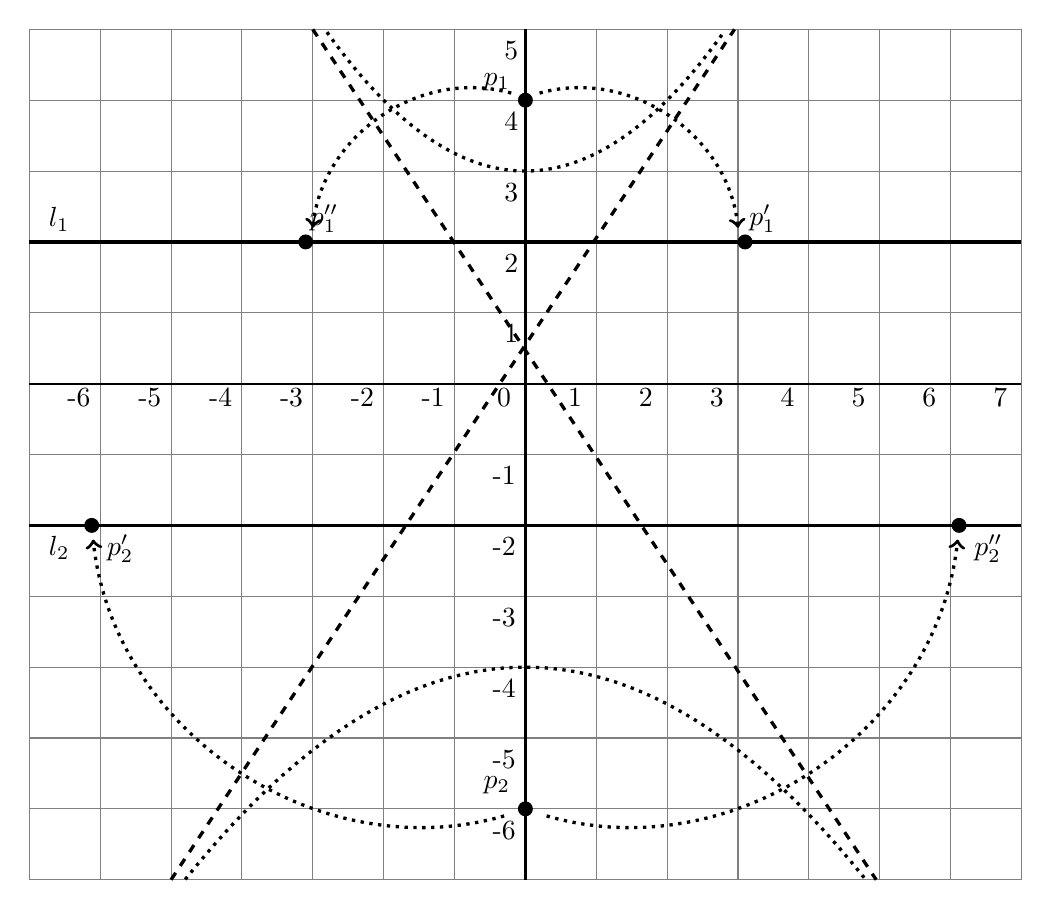
\begin{tikzpicture}[scale=.9]
\draw[step=10mm,white!50!black,thin] (-7,-7) grid (7,5);
\draw[thick] (-7,0) -- (7,0);
\draw[thick] (0,-7) -- (0,5);
\foreach \x in {-6,...,7}
  \node at (\x-.3,-.2) {\sm{\x}};
\foreach \y in {1,...,5}
  \node at (-.2,\y-.3) {\sm{\y}};
\foreach \y in {-6,...,-1}
  \node at (-.3,\y-.3) {\sm{\y}};
  
\coordinate (P1) at (0,4);
\fill (P1) circle (3pt) node[above left,xshift=-2pt] {$p_1$};
\coordinate (P2) at (0,-6);
\fill (P2) circle (3pt) node[above left,xshift=-2pt,yshift=2pt] {$p_2$};

\coordinate (P1P) at (3.1,2);
\fill (P1P) circle (3pt) node[above right,xshift=-2pt] {$p_1'$};
\coordinate (P2P) at (-6.12,-2);
\fill (P2P) circle (3pt) node[below right,xshift=2pt] {$p_2'$};

\coordinate (P1PP) at (-3.1,2);
\fill (P1PP) circle (3pt) node[above right,xshift=-2pt] {$p_1''$};
\coordinate (P2PP) at (6.12,-2);
\fill (P2PP) circle (3pt) node[below right,xshift=2pt] {$p_2''$};

\draw[very thick] (-7,2) -- node[very near start,above,xshift=-34pt] {$l_1$} (7,2);
\draw[very thick] (-7,-2) -- node[very near start,below,xshift=-34pt] {$l_2$} (7,-2);

\draw[domain=-4.8:4.8,samples=50,very thick,dotted] plot (\x,{-.13*\x*\x-4});
\draw[domain=-2.8:2.8,samples=50,very thick,dotted] plot (\x,{.25*\x*\x+3});

\draw[very thick,dashed] (-5,-7) -- (2.95,5);
\draw[very thick,dashed] (-3,5) -- (4.95,-7);

\draw[very thick,dotted,->,bend left=50] (.2,4.1) to (3,2.2);
\draw[very thick,dotted,->,bend left=50] (-.3,-6.1) to (-6.1,-2.2);

\draw[very thick,dotted,->,bend right=50] (-.2,4.1) to (-3,2.2);
\draw[very thick,dotted,->,bend right=50] (.3,-6.1) to (6.1,-2.2);
\end{tikzpicture}
\end{center}
\end{figure}

For a given pair of points and pair of lines, there may be zero, one, two or three folds.

A fold that places $p_i$ onto $l_i$ is a line such that the distance from $p_i$ to the line is equal to the distance from $l_i$ to the line. The locus of points that are equidistant from a point $p_i$ and a line $l_i$ is a parabola with focus $p_i$ and directrix $l_i$. A fold is any line tangent to that parabola. A detailed justification of this claim is given in Appendix~C.

For a fold to simultaneously place $p_1$ onto $l_1$ and $p_2$ onto $l_2$, it must be a tangent common to the two parabolas.

The formula for an arbitrary parabola is quite complex, so we limit the presentation to parabolas with the the $y$-axis as the axis of symmetry. This is not a significant limitation because for any parabola there is a rigid motion that moves the parabola so that its axis of symmetry is the $y$-axis.

An example will also be given where one of the parabolas has the $x$-axis as its axis of symmetry.

\newpage

\textbf{Derivation of the equation a fold}

Let $(0,f)$ be the focus of a parabola with directrix $y=d$. Define $p=f-d$, the signed length of the line segment between the focus and the directrix.\footnote{We have been using the notation $p_i$ for points; the use of $p$ here might be confusing but it is the standard notation. The formal name for $p$ is one-half the \emph{latus rectum}.} If the vertex of the parabola is on the $x$-axis, the equation of the parabola is $y=\disfrac{x^2}{2p}$. To move the parabola up or down the $y$-axis so that its vertex is at $(0,h)$, add $h$ to the equation of the parabola: $y=\disfrac{x^2}{2p}+h$.
\begin{center}
\begin{tikzpicture}[scale=1]
\draw (-6,0) -- node[very near start,below,xshift=-32pt] {$x$-\textsf{axis}}(6,0);
\draw (0,-3) -- node[very near start,right,yshift=-20pt] {$y$-\textsf{axis}}(0,4.5);
\draw[very thick] (-6,-2) -- node[near start,below] {\textsf{directrix} $\quad y=-2$} (6,-2);
\draw[domain=-5:5,samples=50,very thick,dotted] plot (\x,{\x*\x/8+1});
\coordinate (F) at (0,4);
\fill (F) circle (2pt) node[left,xshift=-2pt,yshift=0pt] {$(0,f)=(0,4)$} node[above left,xshift=-2pt,yshift=4pt] {\textsf{focus}};
\fill (0,-2) circle (2pt);
\fill (0,1) circle (2pt) node[below left] {\textsf{vertex}} node[below left,yshift=-10pt] {$(0,1)$};
\draw[<->] (2,-1.9) -- node[fill=white] {$p=6$} +(0,5.8);
\draw[<->] (1,.1) -- node[fill=white] {$h=1$} +(0,.8);
\end{tikzpicture}
\end{center}
Define $a=2ph$ so that the equation of the parabola is:
\begin{form}{1.5}
y=\disfrac{x^2}{2p}+\disfrac{a}{2p}\\
x^2-2py+a=0\,.
\end{form}
The equation of the parabola in the diagram above is:
\begin{form}{1}
x^2-2\cdot 6\,y + 2\cdot 6 \cdot 1=0\\
x^2-12y +12=0\,.
\end{form}
Substitute the equation of an \emph{arbitrary} line $y=mx+b$ into the equation for the parabola to obtain an equation for the points of intersection of the line and the parabola:
\begin{form}{1.5}
x^2-2p(mx+b)+a=0\\
x^2+(-2mp)x+(-2pb+a)=0\,.
\end{form}
The line will be tangent to the parabola iff this quadratic equation has \emph{exactly one} solution iff its discriminant is zero:
\[
(-2mp)^2\:-\:4\cdot 1\cdot (-2pb+a)=0\,,
\]
which simplifies to:
\begin{equation}
m^2p^2+2pb-a=0\,.\label{eq.disc}
\end{equation}

This is the equation with variable $m$ for the slopes of tangents to the parabola. There are an infinite number of tangents because for each $m$, there is some $b$ that makes the line a tangent by moving it up or down.

To obtain the common tangents to both parabolas, the equations for the two parabolas have two unknowns and can be solved for $m$ and $b$.


\textbf{Example}

Parabola 1: focus $(0,4)$, directrix $y=2$, vertex $(0,3)$, $p=2$, $a=2\cdot 2\cdot 3=12$. The equation of the parabola is:
\[
\begin{array}{l}
x^2-2\cdot 2y +12=0\,.
\end{array}
\]
Substituting into Equation~\ref{eq.disc} and simplifying:
\[
m^2+b-3=0\,.
\]
Parabola 2: focus $(0,-4)$, directrix $y=-2$, vertex $(0,-3)$, $p=-2$, $a=2\cdot -2\cdot -3=12$. The equation of the parabola is:
\[
x^2-2\cdot (-2)y+12=0\,.
\]
Substituting into Equation~\ref{eq.disc} and simplifying:
\[
m^2-b-3=0\,.
\]
The solutions of the two equations:
\begin{form}{1.5}
m^2+b-3=0\\
m^2-b-3=0\,,
\end{form}
are $m=\pm\sqrt{3}\approx \pm 1.73$ and $b=0$. There are two common tangents that are the folds:
\[
y=\sqrt{3}x\,,\quad y=-\sqrt{3}x\,.
\]

\textbf{Example}

Parabola 1 is unchanged.

Parabola 2: focus $(0,-6)$, directrix $y=-2$, vertex $(0,-4)$, $p=-4$, $a=2\cdot -4\cdot -4=32$. The equation of the parabola is:
\[
x^2-2\cdot (-4)y +32=0\,.
\]
Substituting into Equation~\ref{eq.disc} and simplifying:
\[
2m^2-b-4=0\,.
\]
The solutions of the two equations:
\begin{form}{1.5}
m^2+b-3=0\\
2m^2-b-4=0\,,
\end{form}
are $m=\pm\sqrt{\disfrac{7}{3}}\approx \pm 1.53$ and $b=\disfrac{2}{3}$. There are two common tangents that are folds:
\[
y=\sqrt{\disfrac{7}{3}}x+\disfrac{2}{3}\,,\quad y=-\sqrt{\disfrac{7}{3}}x+\disfrac{2}{3}\,.
\]

%%%%%%%%%%%%%%%%%%%%%%%%%%%%%%%%%%%%%%%%%%%%%%%%%%%%%%%%%%%%%%%%

\textbf{Example}

Let us now define a parabola whose axis of symmetry is the $x$-axis.

Parabola 1 is unchanged.

Parabola 2: focus $(4,0)$, directrix $x=2$, vertex $(3,0)$, $p=2$, $a=2\cdot 2\cdot 3=12$. The equation of the parabola is:
\[
y^2-4x+12 = 0\,.
\]
Note that this is an equation with $x$ and $y^2$ instead of $x^2$ and $y$, so we can't use Equation~\ref{eq.disc} and we must perform the derivation again.

Substitute the equation for a line:
\begin{form}{1.5}
(mx+b)^2-4x+12=0\\
m^2x^2+(2mb-4)x+(b^2+12)=0\,,
\end{form}
set the discriminant equal to zero and simplify:
\begin{form}{1.5}
(2mb-4)^2\:-\:4m^2(b^2+12)=0\\
-3m^2-mb+1=0\,.
\end{form}
If we try to solve the two equations:
\begin{form}{1.5}
m^2+b-3=0\\
-3m^2-mb+1=0\,,
\end{form}
we obtain a cubic equation with variable $m$:
\begin{equation}
m^3-3m^2-3m+1=0\,.\label{eq.cubic}
\end{equation}
Since a cubic equation has at most three (real) solutions, there can be zero, one, two or three common tangents.

The formula for solving cubic equations is quite complicated, so I used a calculator on the internet and obtained three solutions:
\[
m=3.73\,, \;m=-1\,, \; m=0.27\,.
\]
Choosing $m=0.27$, $b=3-m^2=2.93$, and the equation of the fold is:
\[
y=0.27x+2.93\,.
\]

From the form of Equation~\ref{eq.cubic}, we might guess that $1$ or $-1$ is a root:
\begin{form}{1.4}
1^3-3\cdot 1^2-3\cdot 1+1=-4\\
(-1)^3-3\cdot (-1)^2-3\cdot(-1)+1=0\,.
\end{form}
Divide Equation~\ref{eq.cubic} by $m-(-1)=m+1$ to obtain the quadratic equation $m^2-4m+1$ whose roots are $2\pm\sqrt{3}\approx 3.73, 0.27$.


%%%%%%%%%%%%%%%%%%%%%%%%%%%%%%%%%%%%%%%%%%%%%%%%%%%%%%%%%%%%%%%%

\textbf{Derivation of the equations of the reflections}

For clarity, we derive the position of the reflection $p_1'=(x_1',y_1')$ of $p_1=(x_1,y_1)$ around some tangent line $l_t$ whose equation is $y=m_tx+b_t$. The derivation is identical for any tangent and for $p_2$.

To reflect $p_1$ around $l_t$, we find the line $l_p$ with equation $y=m_px+b_p$ that is perpendicular to $l_t$ and passes through $p_1$;
\begin{form}{2}
y=-\disfrac{1}{m_t}x+b_p\\
y_1=-\disfrac{1}{m_t}x_1+b_p\\
y=\disfrac{-x}{m_t}+\left(y_1+\disfrac{x_1}{m_t}\right)\,.
\end{form}
Next we find the intersection $p_t=(x_t,y_t)$ of $l_t$ and $l_p$:
\begin{form}{3}
m_tx_t+b_t=\disfrac{-x_t}{m_t}+\left(y_1+\disfrac{x_1}{m_t}\right)\\
x_t=\disfrac{\left(y_1+\disfrac{x_1}{m_t}-b_t\right)}{\left(m_t+\disfrac{1}{m_t}\right)}\\
y_t=m_tx_t+b_t\,.
\end{form}
The reflection $p_1'$ is easy to derive because the intersection $p_t$ is the midpoint between $p_1$ and its reflection $p_1'$:
\begin{form}{2}
x_t=\disfrac{x_1+x_1'}{2}\,,\quad y_t=\disfrac{y_1+y_1'}{2}\\
x_1'=2x_t-x_1\,,\quad y_1'=2y_t-y_1\,.
\end{form}

\textbf{Example}

$p_1=(0,4)$, $l_1$ is $y=\sqrt{3}x$:

\begin{form}{2.2}
x_t=\disfrac{\left(4+\disfrac{0}{\sqrt{3}}-0\right)}{\left(\sqrt{3}+\disfrac{1}{\sqrt{3}}\right)}=\sqrt{3}\\
y_t=\sqrt{3}\sqrt{3}+0=3\\
x_1'=2x_t-x_1=2\sqrt{3}-0=2\sqrt{3}\approx 3.46\\
y_1'=2y_t-y_1=2\cdot 3 - 4 = 2\,.
\end{form}

%%%%%%%%%%%%%%%%%%%%%%%%%%%%%%%%%%%%%%%%%%%%%%%%%%%%%%%%%%%%%%%%
\newpage

\section{Axiom 7}\label{s.ax7}

\textbf{Axiom} 
Given one point $p_1$ and two lines $l_1$ and $l_2$, there is a fold $l$ that places $p_1$ onto $l_1$ and is perpendicular to $l_2$.

%\begin{figure}[H]
\begin{center}
\begin{tikzpicture}[scale=1.2]
\draw[step=10mm,white!50!black,thin] (-1,-1) grid (9,8);
\draw[thick] (-1,0) -- (9,0);
\draw[thick] (0,-1) -- (0,8);
\foreach \x in {0,...,9}
  \node at (\x-.2,-.2) {\sm{\x}};
\foreach \y in {1,...,8}
  \node at (-.2,\y-.3) {\sm{\y}};
  
\coordinate (P1) at (5,3);
\fill (P1) circle (2pt) node[below left] {$p_1$};

\coordinate (P1P) at (2.75,5.25);
\fill (P1P) circle (2pt) node[left,xshift=-4pt] {$p_1'$};

\draw[very thick] (1,0) -- node[very near start,right,xshift=2pt] {$l_1$} (3,6);
\draw[very thick,name path=l2] (8,3) -- node[very near start,right,xshift=-2pt,yshift=6pt] {$l_2$} (5,6);

\draw[thick,dotted] ($(1,0)!-.15!(3,6)$) -- ($(1,0)!1.34!(3,6)$);

\draw[thick,dotted] ($(8,3)!-.3!(5,6)$) -- ($(8,3)!1.65!(5,6)$);

\draw[thick,dotted] ($(P1)!-.4!(P1P)$) -- node[very near start,below,yshift=-4pt] {$l_p$} ($(P1)!1.5!(P1P)$);

\draw[very thick,dashed,name path=fold] (-.5,-.25) -- node[very near end,above,xshift=4pt,yshift=6pt] {$l$} (7.5,7.75);

\coordinate (mid) at ($(P1)!.5!(P1P)$);
\fill (mid) circle (2pt) node[below,yshift=-8pt] {$p_m$};

\path [name intersections = {of = fold and l2, by = {perp}}];
\draw[rotate=-45] (mid) rectangle +(8pt,8pt);
\draw[rotate=-45] (perp) rectangle +(8pt,8pt);


\draw[very thick,dotted,->,bend right=50] (5.1,3.2) to (3,5.2);
\end{tikzpicture}
\end{center}
%\end{figure}

\textbf{Derivation of the equation of the fold}

Let $p_1=(x_1,y_1)$, let $l_1$ be $y = m_1x + b_1$ and let $l_2$ be $y=m_2x+b_2$.

Since the fold $l$ is perpendicular to $l_2$, and the line $l_p$ containing $\overline{p_1p_1'}$ is perpendicular to $l$, it follows that $l_p$ parallel to $l_2$:
\[
y=m_2x+b_p\,.
\]
$l_p$ passes through $p_1$ so $y_1=m_2x_1+b_p$ and its equation is:
\[
y=m_2x+(y_1-m_2x_1)\,.
\]
$p_1'=(x_1',y_1')$, the reflection  of $p_1$ around the fold $l$, is the intersection of $l_1$ and $l_p$:
\begin{form}{1.5}
m_1x_1'+b_1=m_2x_1'+(y_1-m_2x_1)\\
x_1'=\disfrac{y_1-m_2x_1-b_1}{m_1-m_2}\\
y_1'=m_1x_i'+b_1\,.
\end{form}
The midpoint $p_m=(x_m,y_m)$ of $l_p$ is on the fold $l$:
\[
(x_m,y_m)=\left(\disfrac{x_1+x_1'}{2},\disfrac{y_1+y_1'}{2}\right)\,.
\]
The equation of the fold $l$ is the perpendicular bisector of $\overline{p_1p_1'}$. First compute the intercept of $l$ which passes through $p_m$:
\begin{form}{2}
y_m=-\disfrac{1}{m_2}x_m+b_m\\
b_m=y_m+\disfrac{x_m}{m_2}\,.
\end{form}
The equation of the fold $l$ is:
\begin{form}{2}
y=-\disfrac{1}{m_2}x+\left(y_m+\disfrac{x_m}{m_2}\right)\,.
\end{form}

\vspace*{-3ex}

\textbf{Example}

Let $p_1=(5,3)$, let $l_1$ be $y=3x-3$ and let $l_2$ be $y=-x+11$.
 

\begin{form}{2.4}
x_1'=\disfrac{3-(-1)\cdot 5-(-3)}{3-(-1)}=\disfrac{11}{4}\\
y_1'=3\cdot \disfrac{11}{4} + (-3)=\disfrac{21}{4}\\
	p_m=\left(\disfrac{5+\disfrac{11}{4}}{2},\disfrac{3+\disfrac{21}{4}}{2}\right)=\left(\disfrac{31}{8},\disfrac{33}{8}\right)\,.
\end{form}
The equation of the fold $l$ is:
\[
y=-\disfrac{1}{-1}\cdot x+\left(\disfrac{33}{8}+\disfrac{\disfrac{31}{8}}{-1}\right)=x+\disfrac{1}{4}\,.
\]

